
Lo scopo di questo capitolo è quello di riassumere gli esperimenti condotti.\newline
\indent Una volta individuati i tool capaci di determinare bound espliciti ai consumi di gas si è testato il loro comportamento su input diversi. Per dedurre la completezza del software, i programmi in input sono stati scelti in modo da testare diversi costrutti base messi a disposizione dal linguaggio Solidity.\newline
\indent I test sono stati condotti con il tool GASTAP e con il compilatore solc, ad oggi gli unici capaci di produrre dei bound ai consumi di gas per gli smart contract di Ethereum. Per quanto riguarda il primo gli sviluppatori hanno fornito i dettagli della sua implementazione, documentando in che modo venga condotta la loro analisi. Conoscere le tecniche utilizzate ha permesso di dedurre alcune proprietà del tool e dell'analisi di smart contract in generale. Dall'altro lato la documentazione ~\cite{solidity-docs} del compilatore solc tratta l'analisi del gas in modo superficiale. Tuttavia il suo impiego nei test condotti ci ha permesso di confrontare i risultati di GASTAP, in modo da considerare l'analisi degli smart contract in chiave critica.\newline

\newpage

\section{Stimare i Consumi di gas}


	\textbf{Perché stimare i consumi di gas è importante?}\newline
    \newline
	\indent I consumi di gas sono associati alle operazioni di basso livello, 
	dunque specificati solo per il bytecode EVM \cite{wood2014ethereum}. Dal momento che però gli
	smart contract sono sviluppati utilizzando linguaggi di alto livello (come
	ad es. Solidity \cite{ethereum/solidity_2019}), è difficile per lo sviluppatore conoscere i 
	costi del proprio programma durante la fase di sviluppo. Per di più la traduzione 
	dei costrutti di alto livello in bytecode fa sì che stimare i constumi tramite l'analisi 
	statica sia una sfida non triviale. L'impiego dell'analisi statica si rende indispensabile, in quanto il costo totale in gas richiesto per eseguire un programma dipende anche da altri fattori.\newline
	\indent Semplificando potremmo dire che i costi totali dipendono da:
	\begin{enumerate}
	\item il costo intrinseco di ciascuna istruzione di basso livello; questi valori sono fissati (vedi Tabella \ref{tab:gas-costs}).
	\item i costi determinati dalla creazione di un contratto o dalla chiamata di un altro programma. Questi sono determinati dalle istruzioni \texttt{CREATE} , \texttt{CALL} and \texttt{CALLCODE}.
	\item eventuali costi aggiunti, che vengono addebitati nel caso in cui la memoria richiesta dal programma superi una certa soglia.
	\end{enumerate}

	Mentre alcuni di questi valori possono essere facilmente stimati, altri possono essere determinati soltanto durante l'esecuzione del contratto. Un modo per sopperire a questa difficoltà è l'analisi statica: soltanto delle tecniche precise ci permettono di stimare questi valori, poichè consentono di calcolare in anticipo quali ``sorprese'' riserverà il codice durante la sua esecuzione.\newline
	\indent Dal momento che il gas viene pagato anticipatamente, può succedere che durante la sua
	esecuzione un programma ecceda la quantità che ha a disposizione. Come conseguenza, la EVM
	sollleva un'eccezione di tipo \textit{out-of-gas} e abortisce la transazione. Un contratto
	che non gestisce bene l'eventuale interruzione di una transazione è soggetto ad una 
	vulnerabilità legata al gas. Una panoramica su questo tipo di vulnerabilità viene fornita dagli autori di \textsc{MadMax} ~\cite{grech2018madmax}. Generalmente questi programmi, che vengono etichettati
	come rischiosi, saranno bloccati in modo permanente.
	Quando si eccede il gas disponibile un'altra conseguenza più immediata è il
	blocco della transazione: la computazione non giunge a termine, l'utente non ottiene il
	risultato desiderato e l'ether pagato per il gas va perso.\newline
	\indent Un altro limite all'esecuzione dei contratti è dovuto al protocollo adottato da Ethereum.
	Questo infatti pone un limite superiore alla quantità di gas che ciascun blocco può consumare. Dal momento che le transazioni vengono raggruppate in blocchi,
	tale limite influenza anche queste: il costo di ciascuna transazione non può superare il limite superiore del blocco al quale appartiene. Può succedere infatti che
	se l'esecuzione di una certa funzione aumenta nel tempo, ad un certo punto non sia
	più possibile portarla avanti a causa del superamento del limite massimo di gas.
	Conoscere a priori i consumi può aiutare anche ad evitare questo tipo di errori.\newline
	\indent Va inoltre considerato che se l'utente della rete ha modo di conoscere il costo
	di una computazione nel suo caso pessimo, ha anche modo di confrontare fra di loro dei programmi
	semanticamente equivalenti, al fine di prediligere quello che consuma meno.  In questo 
	senso la stima dei costi di gas costituirebbe l'uinica fonte di risparmio: considerato
	che le transazioni sotto una certa soglia di \textit{gasPrice} rischiano di non essere 
	accettate dai miner, i committenti non hanno margine di risparmio.\newline
	\indent Una stima affidabile del gas aiuta un utente a stabilire un prezzo per ciascuna
	unità di gas in linea con l'utilità della sua transazione. Infatti una quantità 
	insufficiente per completare la transazione comporta la perdita dei soldi investiti,
	senza che la transazione venga eseguita. Al tempo stesso una sovrastima fa sì che i
	miner assumano un atteggiamento diffidente, abbassando la probabilità che la stessa
	venga scelta.\newline
	\indent Conoscere un limite ai consumi di gas del proprio programma assicura all'utente
	che se la quantità di gas investito supera il bound l'esecuzione verrà portata a termine
	 enza incorrere in spiacevoli sorprese.

	%Si potrebbe aggiungere anche il fatto delle callbak. Quando si chiama un metodo di un altro contratto,e quindi non si conosce lo stato dell'ambiente, poter calcolare i consumi ci permette di mettere a disp una qta di gas adeguata ed eseguire la callback con successo!

	\newpage


\section{Caratteristiche del Tool GASTAP}

GASTAP (acronimo per Gas-Aware Smart contracT Analysis Platform ~\cite{DBLP:journals/corr/abs-1811-10403}), è un tool automatico di analisi statica per i programmi di Ethereum. La principale tecnica di analisi adottata da questo software è la Control Flow Analysis (vedi Sez. 2.2.5).\newline
\indent Dato in input uno smart contract scritto in Solidity, EVM bytecode oppure EVM disassemblato, GASTAP produce un upper bound in termini di gas per ciscuna delle funzioni pubbliche che lo compongono. Per produrre questo calcolo il tool effettua una serie di operazioni in sequenza: (1) costruzione dei grafi \textit{control-flow} (CFG), (2) decompilazione del codice di basso livello in una rappresentazione di alto livello, (3) deduzione delle relazioni di grandezza, (4) generazione delle equazioni di gas, e (5) risoluzione delle equzioni fino a formare un bound.\newline
\indent GASTAP ha un ampio spettro di applicazioni, sia per chi sviluppa o possiede i contratti, sia per gli attaccanti, permettendo di individuare vulnerabilità nel codice e di verificare gli utilizzi di gas, eventualmente anche a scopo di debugging.
Dal punto di vista degli sviluppatori e dei proprietari un buon tool di analisi serve a conoscere la quantità di gas necessaria per eseguire in modo \textit{sicuro} il programma, garantendone la proprietà di liveness. Un altro beneficio è quello di poter determinare quante unità di gas investire per eseguire con successo una callback nei casi in cui uno smart contract si appoggi ad un servizio esterno.
Dal punto di vista degli attaccanti invece è possibile stimare quanto Ether è necessario investire per eseguire un attacco DoS, sebbene tali quantità siano svantaggiose dal punto di vista economico, rendendo poco invitante l'alternativa di compromettere uno smart contract.\newline

    \subsection{Struttura del Tool}
    
    Per implementare ciascuna delle operazioni elencate sopra GASTAP si appoggia ad altri tool open-source. Questi, grazie a degli adattamenti, vengono utilizzati in sequenza al fine di realizzare l'architettura rappresentata in Figura \ref{fig:gstp-struct}.\newline 
    
    \begin{figure}[h]
        \centering
        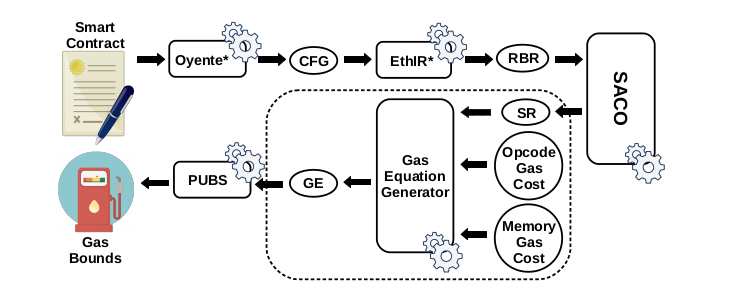
\includegraphics[scale=0.5]{GASTAP-structure.png}
        \caption[Struttura interna di GASTAP]{Architettura di GASTAP}
        \label{fig:gstp-struct}
    \end{figure}
    
    \begin{enumerate}
        \item \textbf{costruzione dei grafi control-flow (CFG)}: tale passaggio è realizzato con \textsc{oyente*}, un'estensione dell'omonimo tool \textsc{oyente} ~\cite{melonproject/oyente}.
        \item \textbf{decompilazione del codice di basso livello}: in questa fase il bytecode viene tradotto in una RBR (\textit{Rule-Based Representation}) grazie ad \textsc{ethir*}, estensione del già citato \textsc{ethir} ~\cite{albert2018ethir}.
        \item \textbf{deduzione delle relazioni di grandezza}: questo passaggio consiste nell'associare a ciascuna delle istruzioni in forma RBR le dimensioni dei dati con i quali interagisce. Quest'operazione è indispensabile per poter costruire le equazioni necessarie a calcolare i bound, e viene realizzata dal tool SACO ~\cite{10.1007/978-3-642-54862-8_46}, che produce le così dette SR (\textit{Size Relations}).
        \item \textbf{generazione delle equazioni di gas}: costituisce il core di GASTAP. Al fine di produrre le equazioni, il tool utilizza le SR insieme alla codifica dei costi delle istruzioni EVM, secondo le specifiche di \cite{wood2014ethereum}. Questi vengono suddivisi tra i costi richiesti dall'esecuzione del bytcode (\textit{Opcode Gas Cost}) e quelli richiesti per l'uso della memoria (\textit{Memory Gas Cost}). 
        \item \textbf{risoluzione delle equazioni fino a formare un bound}: per produrre il risultato finale GASTAP utilizza il solver PUBS ~\cite{albert2008automatic}, che risolve le GE (\textit{Gas Equations}) producendo una formula chiusa dei costi in termini di gas. 
    \end{enumerate}

    \subsection{Interfaccia Web}
    
    GASTAP è utilizzabile tramite un'interfaccia web, disponibile all'indirizzo \\
    https://costa.fdi.ucm.es/gastap.
    
    \begin{figure}[h]
        \centering
        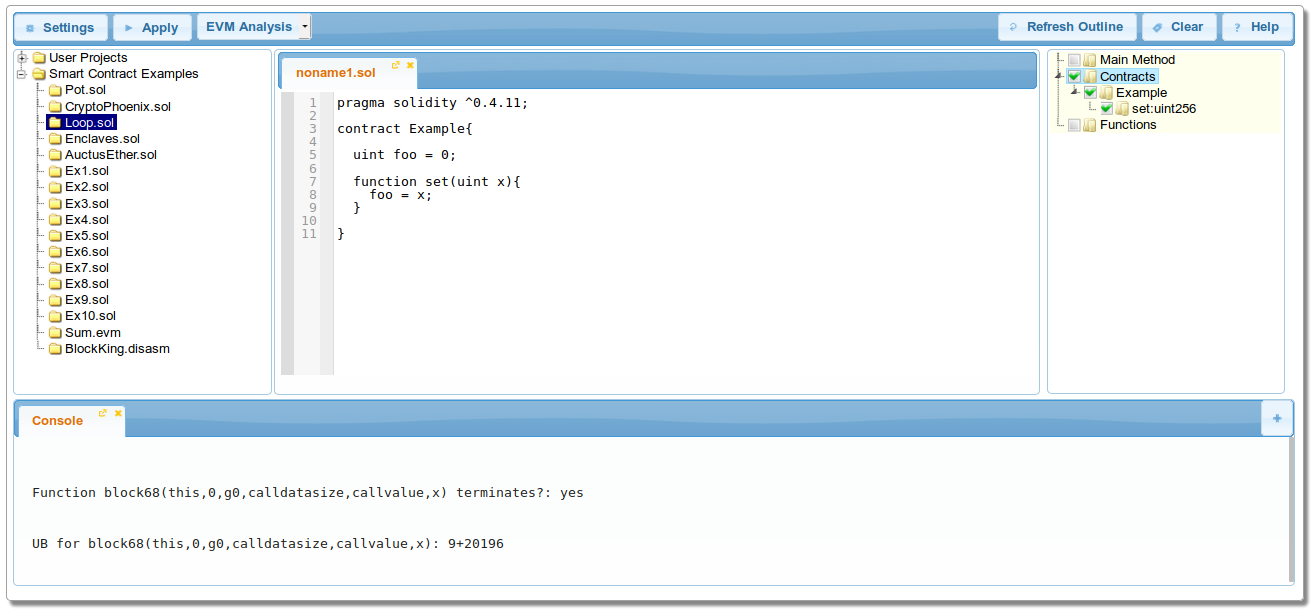
\includegraphics[scale=0.3]{GASTAP-example.png}
        \caption[Interfaccia di GASTAP]{Interfaccia di GASTAP}
        \label{fig:gstp-example}
    \end{figure}
    
    \`E possibile scrivere un proprio programma in Solidity oppure scegliere uno degli esempi proposti dal menù ``Smart Contract Examples''.\newline
    \indent Una volta selezionato il programma di input, cliccando su ``Refresh Outline'' GASTAP mappa le funzioni pubbliche del nostro programma, che vengono mostrate nella sezione di destra. Dopo aver selezionato i metodi che si vogliono analizzare, il pulsante ``Apply'' esegue l'analisi e produce un output nella Console.\newline
    \indent Nell'esempio viene proposto un semplice programma che setta una variabile globale. Stando all'output prodotto, tale programma è garantito teminare, e l'\textit{Upper Bound} (UB) ai consumi di gas è \verb|9+20196|. Si noti che l'upper bound fornito è sempre nella forma \textbf{memory bound} + \textbf{opcode bound}, dove le cifre si riferiscono rispettivamente al bound dei costi di memorizzazione e a quello dei costi delle operazioni che compongono il programma.\newline

    
    
\section{Compilatore solc}

Si tratta del compilatore ufficiale del linguaggio Solidity, utilizzabile da linea di comando.\newline
\indent Il comando \verb|solc --help| fornisce la spiegazione di ciascuna delle opzioni con cui può essere lanciato.

\lstset{
    style=cmd-line,
    literate={~} {$\sim$}{1}
}

\begin{lstlisting}
$~solc --help

solc, the Solidity commandline compiler.

This program comes with ABSOLUTELY NO WARRANTY. This is free software, and you
are welcome to redistribute it under certain conditions. See 'solc --license'
for details.

Usage: solc [options] [input_file...]

...

Allowed options:
  --help               Show help message and exit.
  --version            Show version and exit.
  --license            Show licensing information and exit.
    
...

  --gas                Print an estimate of the  
                       maximal gas usage for each 
                       function. 
 
\end{lstlisting}



Per condurre i nostri test abbiamo utilizzato il compilatore con l'opzione \verb|--gas|. In questa modalità il compilatore è in grado di determinare soltato dei bound costanti; in tutti gli altri casi produce \verb|infinite| come valore di output.\newline 
\indent Ecco un esempio del suo utilizzo sul programma raffigurato in figura \ref{fig:gstp-example}.

\begin{minipage}{\linewidth}
\begin{lstlisting}
$~solc --gas example.sol 

======= example.sol:Example =======
Gas estimation:
construction:
   5093 + 32800 = 37893
external:
   set(uint256):	20205

\end{lstlisting}
\end{minipage}


Confrontando i risultati ottenuti con quelli prodotti da GASTAP si evince che la stima del gas consumato dalla funzione \verb|set()| corrisponde a quela determinata da solc. Dunque l'uso dell'analisi statica non fa sì che si perda accuratezza nel calcolo.\newline
\indent Nella sezione 4.3.2 l'esempio verrà ripreso al fine di comprendere il bound.\newline


\newpage

\section{Test Condotti}

La nostra analisi è stata condotta su un insieme di programmi scritti in Solidity, disponibili nella repository ~\cite{melastone-sc}.\newline
\indent Ad eccezione di \verb|CryptoPhoenix.sol|, uno degli esempi proposti dal tool GASTAP, gli altri smart contract sono stati sviluppati seguendo la documentazione ufficiale del linguaggio Solidity ~\cite{solidity-docs}. Si tratta di semplici programmi ad hoc per il testing dei costrutti di base del linguaggio di programmazione. Di seguito i casi che abbiamo trattato.\newline

    \subsection{Caso di Studio: CryptoPhoenix.sol}
    %inserire tabella confronti
    %può essere utile?
    
    \subsection{Operazioni di Assegnamento}
    
    I programmi \verb|assignment*.sol| implementano dei contratti che contengono un numero arbitrario di operazioni di assegnamento.
    
    \begin{minipage}{\linewidth}
        \begin{lstlisting}
        //assignment2.sol
        
        pragma solidity ^0.4.11;

        contract B{

            function init(){
                uint number = 1;    
            }

        }

        \end{lstlisting}
    \end{minipage}

    
    Abbiamo potuto verificare come l'operazione di assegnare un valore ad una variabile locale (\verb|assignment2.sol|) o globale (\verb|assignment3.sol|, \verb|assignment4.sol|) costa una quantità di gas relativamente bassa, in media 140 unità.
    Aggiungendo un'operazione di assegnamento in più, che va dunque ad incrementare il valore precedente della variabile, questa stima in alcuni casi subisce una crescita notevole: passiamo da 140 unità a circa 20000.
    
    \begin{minipage}{\linewidth}
        \begin{lstlisting}
        //assignment1.sol
        
        pragma solidity ^0.4.11;

        contract A{

            uint number = 0;

            function init(){
                number = 1;    
            }

        }

        \end{lstlisting} 
    \end{minipage}

    
    Tale incremento è dato dalla presenza nel codice EVM dell'istruzione SSTORE (vedi Tabella \ref{tab:gas-costs}). Si evince dunque che la semplice operazione di settare il valore di una variabile da 0 ad uno diverso da 0 ha un impatto notevole sulla performance del programma in termini di costi. Un caso simile si era verificato nel caso del programma \verb|example.sol|.

    \subsection{Costrutto for}
    
    Testando i cicli for si è ottenuto un risultato interessante. La compilazione di questi programmi con solc produce sempre un bound infinito. Al contrario i test con GASTAP hanno prodotto una stima finita dei consumi.\newline
    
     
    \begin{minipage}{\linewidth}
    \begin{lstlisting}
    //loop1.sol
    //esegue la moltiplicazione di number*a

    pragma solidity ^0.4.11;

    contract Loop1{

        uint sum = 0;
        uint number;
        
        function multiply(uint a){
            
            for(uint i = 0; i<a; i++){
            sum = sum+number;
            }
        }

    }
    \end{lstlisting}
    \end{minipage}

    
    Gli output ottenuti con solc e GASTAP sono, rispettivamente:
    
    \begin{minipage}{\linewidth}
    \begin{lstlisting}
    ======= loop1.sol:Loop1 =======
    Gas estimation:
    construction:
    5099 + 39200 = 44299
    external:
    multiply(uint256):	infinite
    \end{lstlisting}
    \end{minipage}

    
    e
    
    \verb|GASTAP: 9+ (222+20476*nat(a))|
    
     
    \begin{minipage}{\linewidth}
    \begin{lstlisting}
    //loop2.sol
    //somma i primi 10 elementi di un vettore

    pragma solidity ^0.4.11;

    contract Loop2 {

        function sum (uint[] nums) returns (uint sol) {
            sol = 0;
            for(uint i = 0; i < 10; i++)
                    sol = sol+nums[i];
            }

    }
    \end{lstlisting}
    \end{minipage}

    
    Gli output ottenuti con solc e GASTAP sono, rispettivamente:
    
    \begin{minipage}{\linewidth}
    \begin{lstlisting}
    ======= loop2.sol:Loop2 =======
    Gas estimation:
    construction:
    111 + 59200 = 59311
    external:
    sum(uint256[]):	infinite
    \end{lstlisting}
    \end{minipage}

    
    e
    
    \verb|GASTAP: 3*max([4+nat(nums)+1,4+nat(nums)+2])+pow(max([4+nat(nums)+1,4+nat(nums)+2]),2)/512+ (1746+3* (1/32))|
    
    Come si può evincere da quest'ultimo caso gli upper bound forniti da GASTAP possono essere parametrici. Nell'esempio il parametro è determinato dal valore in input di una delle funzioni pubbliche del contratto.\newline
    \indent Più in generale possiamo dire che l'output prodotto da GASTAP è parametrico:
    \begin{itemize}
     \item nella dimensione dei parametri delle funzioni
     \item nello stato del contratto
     \item nei dati della blockchain dai quali dipendono i cosumi di gas (es. valore dell'ether)
    \end{itemize}


    
    \subsection{Cicli for Annidati}
    
    Per verificare la gestione dei cicli for annidati si è implementato un semplice programma che attraverso il metodo \verb|suma(uint a)| esegue \verb|a| incrementi della variabile locale \verb|sum| attraverso un ciclo for.
    
    \begin{minipage}{\linewidth}
    \begin{lstlisting}
    //nested1.sol

    pragma solidity ^0.4.11;

    contract Nested1 {

        uint total_loops;

        // restituisce un valore uguale ad a, ottenuto sommando a volte 1.
        // ad ogni iterazione incrementa la var total_loops.
        function suma (uint a) returns (uint sum) {
            sum = 0;
            for(uint i = 0; i < a; i++)
                    sum = sum+1;
                    total_loops = total_loops +1;          
        }

    }
    \end{lstlisting}
    \end{minipage}

    
    Il programma è stato modificato in successione, inserendo un ciclo for annidato alla volta all'interno di \verb|suma(uint a)|. Ad ogni incremento abbiamo nuovamente calcolato il bound alla funzione \verb|suma(uint a)| con entrambi i programmi. Denotiamo con la variabile n il livello di annidamento dei cicli for. I risultati ottenuti sono mostrati nella Tabella \ref{tab:nested-outputs}.
    
    \begin{table}[h]
    \begin{threeparttable}[b]
     


     \begin{center}
        \caption[legenda elenco tabelle]{Risultati dell'analisi dei programmi nested*.sol}\label{tab:nested-outputs}
        \begin{tabular}{ccp{12cm}}  
        \hline \hline   %inserisce due righe orizzontali
        $n$ & solc & GASTAP \\   %& separa le colonne
        \hline  %inserisce una riga orizzontale
        \bf1 & infinite & $15 + (20508+70*nat$\tnote{1}$(a))$\\
        \bf2 & infinite & $15 + (20548+70*nat(a)+20276*nat(a))$\\
        \bf3 & infinite & $15 + (20588+70*nat(a)+20276*nat(a)+20276*nat(a))$\\
        \bf4 & infinite & $15 + (20628+70*nat(a)+20276*nat(a)+20276*nat(a)+20276*nat(a))$\\
        \end{tabular}
        \begin{tablenotes}
            \item [1] La funzione nat è definita come nat(l)=max(0,l)
        \end{tablenotes}
     \end{center}
    \end{threeparttable}
    \end{table}

    
    Continuando ad incrementare il numero di cicli, si è potuto dare un bound al livello di annidamento. Per $n$ = 15 GASTAP non riesce a mappare le funzioni nella outline. Questo implica che non può essere condotta l'analisi sul programma \verb|nested15.sol|. Il limite dunque è dato dalla struttura del codice. L'esempio è mostrato in Figura \ref{fig:gstp-nested15}\newline
    
    \begin{figure}[h]
        \centering
        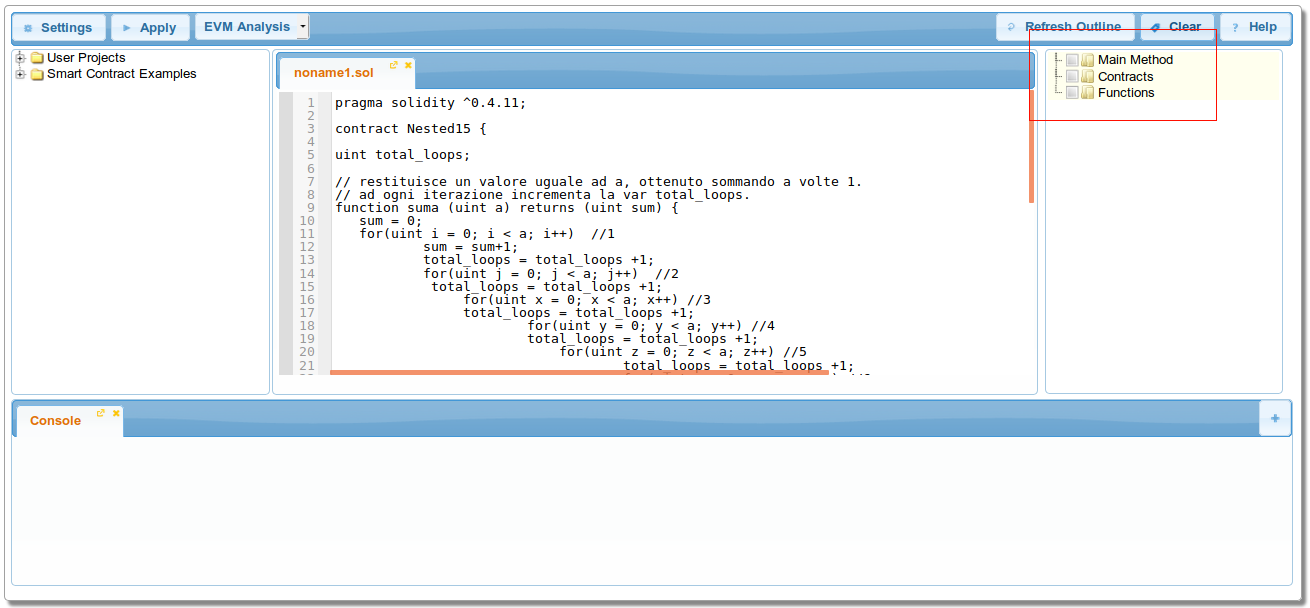
\includegraphics[scale=0.3]{GASTAP-nested15.png}
        \caption{nested15.sol in GASTAP}
        \label{fig:gstp-nested15}
    \end{figure}

    \begin{minipage}{\linewidth}
    \indent Dai risultati ottenuti conducendo i nostri test è stato possibile ricavare la seguente formula di ricorrenza per il bound determinato da GASTAP per i programmi nested$n$.sol:
    \[ \forall 0 < n \leq 14 \quad \mathrm{UB} = 15 + (20508 + (n - 1)*40 + 70*nat(a) + (n - 1)*20276*nat(a)) \]
    \end{minipage}

    \subsection{Costrutto while}
    
        \subsubsection{while.sol}

        \subsubsection{sqrt.sol}

    \subsection{Ricorsione}

        \subsubsection{Ricorsione Diretta}

        \subsubsection{Ricorsione Indiretta}
        
        \subsubsection{Ricorsione Multipla}
    
\section{Risultati}

